\chapter{Background}
\todo{write introdction}
\todo{check whether following sections make sense }

\section{Secure Cloud Storage System}
In the past 20 years we witnessed a shift of resource consumption on the user side to outsourcing more and more resources into the cloud. Naturally, users moved their files into cloud storage systems. This helped companies to maintain an ecosystem around the user helping him to synchronize his files onto different devices.  

With increasing transparency raised also the concern that it was not clear anymore who could access the private files especially when they are transmitted and stored on oversee servers. Bdrive, a secure cloud storage system, committed to not export files and data to other countries. It splits up files in smaller chunks that are saved separately on different cloud storage provider (\ac{CSP}). To ensure end-to-end encryption a Bdrive client encrypts locally each of its chunks with a one-time symmetric key that is then encrypted under its own public key. This encrypted key is called a file key and it is uploaded to the Bdrive server where it is stored securely, as shown in Figure \ref{fig:filekey}.

\section{Background}
\label{sec:background}
\begin{figure*}[!ht]
\centering
    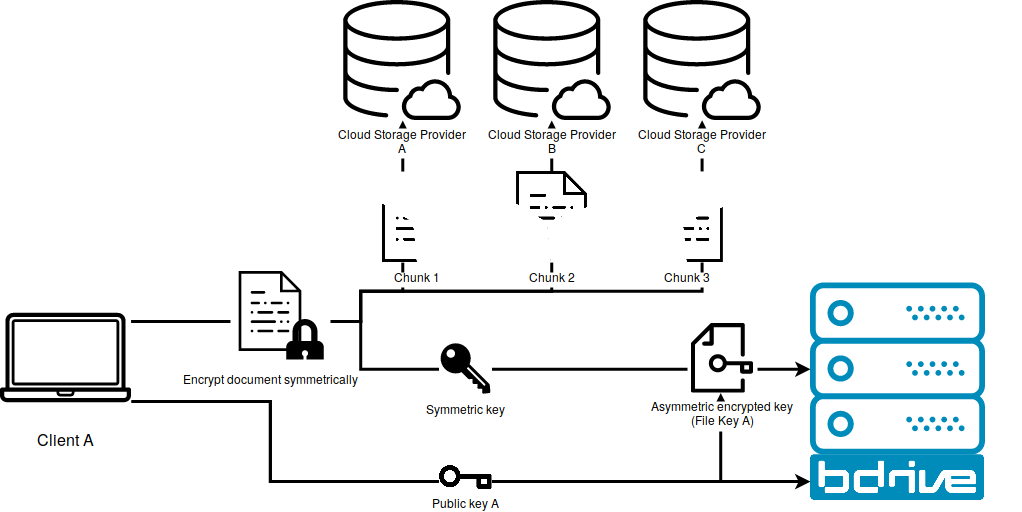
\includegraphics[width=1\linewidth]{img/bdrive1.png}\par 
    \caption{Device uploads an encrypted file to the \ac{CSP}s and the file key and public key to Bdrive.}
    \label{fig:filekey}
\end{figure*}
\begin{figure*}[!ht]
\centering
    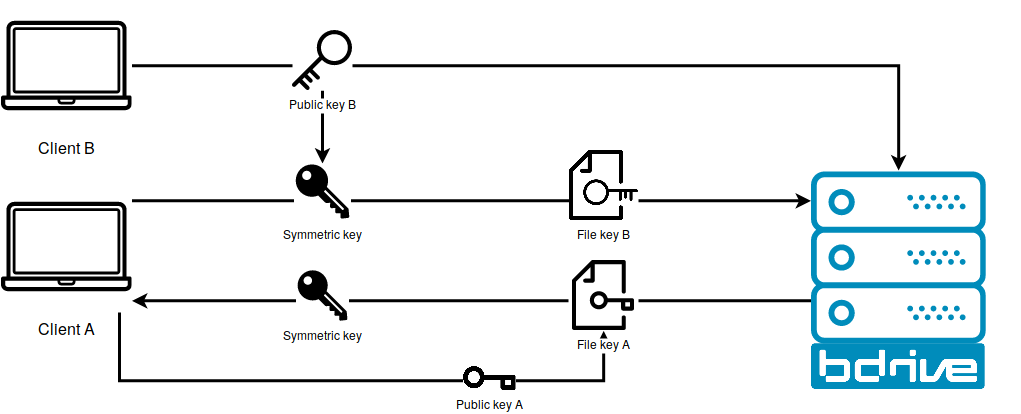
\includegraphics[width=1\linewidth]{img/bdrive2.png}\par
    \caption{Device A grants Device B access to the uploaded file by re-keying the file key}
    \label{fig:rekey}
\end{figure*}
Since each device of the same user has its own private-public key pair, an existing device is in charge of making its accessible file keys available for a new device. This will be done by downloading each file key for the respective file, receiving the public key of the new device, decrypting the file key with its own private key, encrypting it again with the public key of the new device and finally, uploading the new file key to the Bdrive server. This process will be called re-keying, as shown in Figure \ref{fig:rekey}. 

% File upload and file key creation
In Bdrive each device of a user generates a new \ac{RSA} key pair on registration. The fingerprint (SHA-1 or MD5 hash) of the public key identifies the device uniquely. To save a file in the cloud the device first encrypts the file symmetrically with the so called "filekey". The filekey equals the hash of the plain file content and so ensures tamperproofness and integrity on decryption. End-to-end encryption implies that the server should never be able to decrypt the file by itself. To enforce this the device encrypts the filekey asymmetrically with its own public key before uploading the filekey to the Bdrive server where it is stored securely. In Bdrive, the encrypted file chunks are uploaded to the different cloud storage provider (\ac{CSP}). 

% Access file
If the user wants to access a file locally, the devices requests the encrypted filekey from the server and downloads the file chunks from the \ac{CSP}s. Locally, it decrypts the filekey with his private key and finally deciphers the assembled file with the decrypted filekey. 

% Process for multibe devices
So far the encryption process for a single device has been outlined. However, this process turns out to be much more computationally complex in a multiple device setting.  If a user registers more then one device the existing data needs to be synchronized to the new device. The server notifies the existing device for the newly registered one and the public key of the new device is downloaded. Now the existing device needs to download each filekey for each file of the user and decrypts it. The synchronization is finished by encrypting the filekeys with the new devices public key and uploaded again to the server. The new device can now start to download and decrypt the file chunks as described previously.

Usually in cloud storage systems we also have the concept of groups. They describe a collection of clients which share data between them. For that they form a so called \textit{share}. To express the overhead of joining or leaving a share the following notation will be used: $f$ and $n$ donate the number of filekeys and the number of devices in a share respectively.

% Adventages
If a new devices joins a share in Bdrive a device needs to make the existing file keys available to the new devices which results in $f$ additional encryptions, messages and keys. However, a big advantage of this scheme is that forward secrecy\footnote{Forward Secrecy: The left entity will have no knowledge about future shared content.} will not produce additional overhead. Here, only all the filekeys belonging to the left device are removed and the other devices do not further encrypt new uploaded files for this device anymore. The backward secrecy constrain, while being an imported security feature, will explicitly be broken by clients. This is due to the feature, that data owner can invite a new member into a group and the new member accesses all previous uploaded content. Bdrive is ensuring this by explicitly reencrypting all file keys for the new device. 

\section{Problem Description}
% Bdrive rekeying
% Motivation and Problem description

% Disadventages in shares
Notice, that this approach is not scalable for a large number of devices. To showcase this, the use case of creating a new share is analyzed. Each device invited to a share needs to have an own version of the file key, encrypted with the devices public key, issued. This process scales with $O(n * f)$ keys. 
%Were $n$ donates the number of devices involved in the sharing and $f$ the number of file versions in the share.\footnote{Each file consist of many file versions. Each file version needs an own file key since for each content change a new file is updated.}
Further, the same number of messages containing the encrypted file key need to be send and each filekey needs to be encrypted $n$ times which also results in $O(n * f)$ encryptions in total. 

To make the overhead more clear, lets assume a manager of a company with 50 employees who wants to create a company wide share. Each of the employees has at least two devices (say one web view client and a desktop client). To upload the latest presentation the device of the manager know has to create $50 * 2 = 100$ filekeys to upload, $100-1$ messages, containing encrypted file key for each device, to distribute and $100$ encryptions to make. Even worst for each new presentation upload another $100$ filekeys need to be maintained. In a large scale company this overhead becomes unmaintainable when the number of $10.000$ filekeys are exceeded. \footnote{Running 'openssl speed rsa1024' on an Intel(R) Core(TM) i7-6500U CPU @ 2.50GHz takes on average 0.000113s for encryption. Multiplied by 10.000 the second mark is reached.} With increasing computing power this problem can be compensated but not prevented.

\section{Attribute-Based encryption}
\label{sec:attribute-based-encryption}
\textit{Attribute-Based Encryption} (\ac{ABE}) defines users over attributes and attribute keys rather then its individual public key. Since users are not unique among their attribute set it is possible to reduce the number of needed keys of a share to the number of attributes necessary to describe the group completely. 

In the previous example the manager would only need to encrypted the presentation one time: With the public key of the attribute “working in company”. In this participial use case only $1$ encryption is done, $1$ message is distributed using multi-cast to transmit same encrypted file to all clients, and $1$ file key is created. 

Of course this advantage does come at some cost. While classical encryption schemes provide complete End-to-End encryption, ABE needs a \textit{Attribute Authority} (\ac{AA}) to issue attribute and attribute keys in the first place. This authority has global decryption power in the administered domain. For that reason the attributes need to be split up into different domains, each managed by an own AA. In the use case of cloud storage systems for business it makes sense to setup an AA for each company. 

With ABE comes the advantage of defining access policies for cipher texts. This policies consist of boolean formulas with attribute values as inputs. Only if a user satisfies the given policy he is able to decipher the cipher text. The use of this access formulas helps to eliminate authorization checks, since clients can either decrypt the file and are therefor allowed to access the plaintext or they are not able to decrypt and so do not satisfy the given policy. 

% In our use case inter company sharing becomes tricky. Now different AAs need to cooperate to create cipher text policies containing attributes of the whole ecosystem.  

ABE scales with the number of attributes contained in a cipher text. As long as a group can be described with less attributes then there are members in this group, a better performance of ABE compared to the current scheme in Bdrive can be achieved. 

ABE comes in many different favors. The most important for this work are Single-Authority Attribute-Based Encryption (normal \ac{ABE}) and Multi-Authority Attribute-Based Encryption (\ac{MA-ABE}). 
For the single authority use case three entities are defined:

\begin{enumerate}
	\item \textbf{Attribute Authority (\ac{AA});} An attribute authority issues user their unique identifier (\ac{UID}), attributes and their respective attribute secret keys. 
	On revocation the AA will need to update the users secret keys as well as the ciphertext encrypted with the revoked attribute key. 
	Since an AA always generates the private attribute key to derivate a new user specific secret key it has global decryption power. That’s why the single-authority use case the AA is assumed to be an trusted entity. 
	\item \textbf{Cloud Storage Provider (\ac{CSP});} The cloud storage provider are assumed to be untrusted but they still follow the protocol. That’s why they only receive encrypted data. They only purpose is to store the ciphertext and make them permanently available. Since the authorization to each ciphertext is directly embedded into the cipher-text access policy, the download of the encrypted file does not need any authentication checks.
	\item \textbf{Users/Data Owners;} Users exist in two groups: Revoked and non-revoked. Non-revoked users try to collude with each other to get a higher level of decryption power. They download the files of the \ac{CSP} and try to decrypt them. Only if they attribute set matches the policy of the ciphertext they will be able to decrypt the file. 
	Revoked users, on the other hand, try to still decipher ciphertext. In some cases they try to collude with non-revoked user to intercept the key update key to restore their decryption rights. 
	User are in general untrusted.

	Users (some schemes differentiate between decrypting users and encrypting data owners) want to encrypt content with a specific access policy. To do so they use the public available public attribute keys pinned on the bulletin board of the \ac{AA}. They do not have to know anything about the receiving user or user groups in the system. After encryption they update the encrypted content to the \ac{CSP}.
\end{enumerate} 

MA-ABE states the following adaptation and additions:

\begin{enumerate}
	\item \textbf{Attribute Authority (\ac{AA});} In the system of MA-ABE there are multiple AAs. Each administrating their own domain. AAs are usually assumed to be honest-but curios. They distrust each other and try to decrypt files of other domains. A big goal for MA-ABE is to achieve inter-authority communication so that cipher-texts can ce encrypted using different attributes of different domains. An AA still bootstraps its users, but can also issue external users attributes.
	\item \textbf{Certificate/Central Authority (\ac{CA});} The purpose of the \ac{CA} is to issue user their global identifier (\ac{GID}). This GID is unique among the whole user universe and identify a user uniquely against each AA. Further, it bootstraps the different \ac{AA}s. The \ac{CA} usually remains trusted but. In many MA-ABE schemes the CA has global decryption power. The CA can also act as an \textit{Certificate Authority} to make users as valid participants in the system. If central authority and certificate authority have different trust levels, they are modeled as different entities.
	\item \textbf{Server;} Some schemes additional introduce a server. Its task is it to help user with proxy re- and decryption. If an \ac{AA} broadcasts a revocation of an attribute, the server downloads all related ciphertexts from the \ac{CSP} to update them with the new attribute. 
	The thread model for the server is honest-but-curious or even untrusted. Please note, that the \ac{CA} and the server are two separated entities that do not cooperate.
\end{enumerate} 

Users and CSP remain unchanged in the MA-ABE case.

\section{Thread Model}
\label{sec:thread-model}
MA-ABE describes six entities which will have different trust levels in the design. In the following the certificate authority and central authority, as well as the user and data owners are merged. For the goal of this work the thread model and different trust level of the entities are defined as:

\begin{itemize}
	\item The \textbf{Central Authority} is assumed to try to break into the client communication. It might provide false information or wrong states to trick any identity to provide sensitive content. However, the central authority will cooperate and will only deviate from the protocol if some advantage could be gained. Simply denying the cooperation - and so disrupting the service - does not belong to the goals of the central service. The central service does not cooperate with other malicious entities. 
	\item Each \textbf{Attribute Authority}’s goal is to access and eve drop content that is encrypted with attributes outside if its domain. This distrust can be leveraged by a trust relation ship, where two attribute authorities can explicitly agree to trust each other. This mutual trust relation indicates that an trusted attribute authority is assumed to provide only truthfully information to the other trusted authority. Again it is assumed that an attribute authority does not cooperate with other malicious entities and that it will follow the protocol.
	\item \textbf{Cloud Storage Provider} are simply assumed to be honest-but-curious. They follow the protocol by try to decrypt content if possible. A cloud storage provider is separated from the other system and does not cooperate with any other malicious entity.  
	\item \textbf{Users} are untrusted. They try to collude with each other to achieve a higher level of decryption power. That means that they will exchange private attribute and two factor keys (see Section \ref{sec:dac-macs}). However, it is assumed that they will not sell a decryption black box so that other external, unauthorized or revoked users use the black box to access sensitive content. 
\end{itemize}

This thread model was adapted from that in TF-DAC-MACS \cite{li2017two}. Here the central authority and certificate authority are also semi-trusted. This is compensated by leveraging the trust level of the attribute authorities by introducing the trust-relationship. In TF-DAC-MACS a lot of trust is rooted in the certificate which was issued by the trusted certificate authority. In a real life system the trust of the certificate authority needs to be deescalated, since it is usually controlled by the same entity as the central authority or at least act on its behave. To do so, for each certificate validation a second channel needs to be established: One to the issuer and one to the subject of the certificate, asking both for the validity of the certificate. 

\section{Requirements}
\label{sec:requirements}
Based on the previous introduced entities in ABE \ref{sec:attribute-based-encryption}, the thread model \ref{sec:thread-model} and the security requirements of a secure-cloud storage system the following requirements can be extracted.

The general (\req{B}) requirements of this thesis will be summarized by two major points: 

\begin{itemize}
	\item[\req{B1}] \textbf{Performance:} Participating in the system should be possible with low-performance devices (such as smartphones). The overhead for the server on proxy decryption, attribute issuing and revocation should be reasonably low.  
	\item[\req{B2}] \textbf{Scalability:} The system should scale better than the current encryption scheme with respect to the number of file keys. This summarizes the performance impact of a growing number of clients.
\end{itemize}

In addition, the core (\textbf{\textit{C*}}) security requirements in the context of an \ac{MA-ABE} scheme are the following:
\begin{itemize}
\item[\req{C1}] \textbf{Collusion resistance:} For two users it should not be possible to combine their attributes to achieve a higher level of decryption power. Collusion resistance need also be ensured also on revocation. 
\item[\req{C2}] \textbf{Inter-Company Sharing:} Each company is only responsible for its own domain. This includes attribute and user administration, which translates to secret key generation and revocation. 
\item[\req{C3}] \textbf{Central Authority:} The Central Authority (\ac{CA}) shall not have global decryption power. At most an Attribute Authority (\ac{AA}) can decrypt user files of its own domain.  
\item[\req{C4}] \textbf{Secret Master key (if any):} Key recovery requires a secret and securely stored master key. It should solely function in the company domain and not globally. 
\item[\req{C5}] \textbf{Large Attribute and Key Universe:} The number of attributes and users shall not be restricted.
\item[\req{C6}] \textbf{Adding new Attribute Authorities:} It should be possible to add new AAs at runtime. Without either shutting down the system or recreating each key.
\item[\req{C7}] \textbf{Untrusted Attribute Authority:} A corrupt AA can only harm its own domain, but can not harm the outside system in any way. It cannot gain any additional information.
\item[\req{C8}] \textbf{Key and Attribute revocation:} Revocation is needed to handle user management in terms of attribute promotion, attribute demotion and key revocation. Forward secrecy should be provided.
\end{itemize}

\noindent Other (optional \textbf{\textit{O*}}) requirements are: 
\begin{itemize}
	\item[\req{O1}] \textbf{Traitor tracing:} A user in \ac{ABE} is described by his attribute set and is anonymous in this set. Misbehaving users, who sell their attribute keys to create a decryption black box, should be identifyable \cite{liu2016practical}.
	\item[\req{O2}] \textbf{Fine-grained access control:} The user shall not be bounded on defining fine-grained access policies which requires either an access tree \cite{bethencourt2007ciphertext} or an linear secret sharing scheme (\ac{LSSS}) \cite{yang2013dac} \cite{li2016secure} \cite{wu2017security} \cite{li2013matrix} \cite{liu2016practical}.
	%Some schemes restrict the user to threshhold access policies, where a user needs at least $n$ of $m$ attributes to encrypt the cipher text. \cite{chase2007multi} \cite{chase2009improving} Other approaches are restriced to $\ac{AND}$ gates which would translate to $m$ of $m$ threshhold gates. \cite{li2017two}
\end{itemize}

\section{Contribution}
In this work different schemes suitable to resolve the rekeying problem will be compared. First, the group communication schemes on a theoretical bases are compared. Then it is argued why ABE might scale even better and different schemes are compared on a practical level. To do so a homogeneous platform was used and different benchmarks will be performed to evaluate the performance and scalability of thous schemes. Thous benchmarks are novel in that matter that no other research compared the different ABE topics on a practical level.  

In the second part of this work, an prototype implementation of the selected approach will be given which will stay as close as possible to the current scheme in Bdrive. To make the selected scheme practically applicable and to fit the requirements of section \ref{sec:requirements}, small adaptation to the scheme will be made. The target will be to compare the current scheme and the ABE approach. Further, a conclusion of the applicability of ABE in the real world is drawn and it is evaluated whether ABE does also scale better in real life scenarios. 